\documentclass[conference]{IEEEtran}
\IEEEoverridecommandlockouts
% The preceding line is only needed to identify funding in the first footnote. If that is unneeded, please comment it out.
\usepackage{cite}
\usepackage{caption}
\usepackage{amsmath,amssymb,amsfonts}
\usepackage{algorithmic}
\usepackage{multirow}
\usepackage{hhline}
\usepackage{graphicx}
\usepackage{textcomp}
\usepackage{xcolor}
\usepackage{graphicx} % Required for inserting images
\def\BibTeX{{\rm B\kern-.05em{\sc i\kern-.025em b}\kern-.08em
    T\kern-.1667em\lower.7ex\hbox{E}\kern-.125emX}}

\title
    {
        Implementasi Teknologi Pengenalan Gambar Untuk Meningkatkan Keamanan Sistem Komputer Dengan Mendeteksi Dan Mengidentifikasi Wajah
    }

\author{\IEEEauthorblockN{1\textsuperscript{st} Andrew Thomas Agustinus}
\IEEEauthorblockA{\textit{Fakultas Teknik dan Informatika(of Aff.)} \\
\textit{Universitas Multimedia Nusantara(of Aff.)}\\
Tangerang, Indonesia\\
andrew.thomas@student.umn.ac.id}
\and
\IEEEauthorblockN{2\textsuperscript{nd} Arvin Winardi}
\IEEEauthorblockA{\textit{Fakultas Teknik dan Informatika (of Aff.)} \\
\textit{Universitas Multimedia Nusantara(of Aff.)}\\
Tangerang, Indonesia\\
arvin.winardi@student.umn.ac.id}
\and
\IEEEauthorblockN{3\textsuperscript{rd} Axel Ferdinand}
\IEEEauthorblockA{\textit{Fakultas Teknik dan Informatika(of Aff.)} \\
\textit{Universitas Multimedia Nusantara(of Aff.)}\\
Tangerang, Indonesia\\
axel.ferdinand@student.umn.ac.id}
\and
\IEEEauthorblockN{4\textsuperscript{th} Mohammad Alfarizky Ramadhani Oscandar}
\IEEEauthorblockA{\textit{Fakultas Teknik dan Informatika(of Aff.)} \\
\textit{Universitas Multimedia Nusantara(of Aff.)}\\
Tangerang, Indonesia\\
mohammad.alfarizky@student.umn.ac.id}
}
\date{May 2023}

\begin{document}

\maketitle

\begin{abstract}
    Pengenalan wajah untuk keamanan komputer menggunakan pendekatan algoritma genetika merupakan solusi menjanjikan dalam era komputasi dan kecerdasan buatan. Metode ini dapat digunakan dalam berbagai bidang keamanan digital, meskipun dihadapkan pada tantangan variasi struktural wajah dan kondisi lingkungan yang kompleks. Penelitian ini menunjukkan bahwa algoritma genetika memiliki potensi yang tinggi dalam meningkatkan tingkat akurasi pengenalan wajah, sebanding dengan metode analisis komponen utama (PCA) dan analisis diskriminan linier (LDA). perlu pertimbangan ketersediaan data variasi wajah yang memadai dan pemilihan parameter pengujian yang tepat guna meningkatkan keakuratan dan kehandalan sistem keamanan biometrik di masa depan.
\end{abstract}

\begin{IEEEkeywords}
Face recognition, computer security, artificial intelligence, genetic algorithm, biometric systems.
\end{IEEEkeywords}

\section{Pendahuluan}
\subsection{Latar Belakang}
Di era digital saat ini, sistem komputer menjadi kebutuhan manusia untuk membantu menyelesaikan berbagai pekerjaan penting dalam kehidupan sehari-hari. Mulai dari komunikasi, menyelesaikan masalah, menjalankan bisnis dan mengelola data menjadikannya sangat dibutuhkan di kehidupan manusia. Peningkatan konektivitas jaringan komputer di dunia memberikan dampak yang berpengaruh untuk kehidupan manusia. Dengan demikian, komputer saat ini tidak hanya dapat membantu manusia untuk menyelesaikan tugas-tugas konvensional seperti komunikasi, mengetik, merangkum informasi, dan lainnya. Namun, komputer saat ini dapat membantu manusia dalam mengambil keputusan dan meringkas pekerjaan-pekerjaan konvensional sebelumnya dengan teknologi kecerdasan buatan. 

Teknologi kecerdasan buatan tidak hanya memberikan dampak yang positif untuk kehidupan manusia. Namun, dengan pesatnya peningkatan kecerdasan buatan juga dapat menimbulkan masalah keamanan di lingkungan digital. Keterbatasan manusia untuk mengolah informasi dan memiliki bias framing dalam mempersepsikan situasi menjadikannya rentan untuk dieksploitasi oleh program-program jahat. Salah satu kemungkinan celah keamanan yang menjadi masalah yaitu program robot yang menirukan manusia untuk mendapatkan keuntungan dalam memproses tindakan yang seharusnya dilakukan oleh manusia. Menurut Gollman keamanan komputer berhubungan dengan pencegahan diri dan deteksi terhadap tindakan pengganggu yang tidak dikenali dalam sistem komputer. \cite{Adrianto2016}. Dengan demikian, diperlukan adaptasi kecerdasan buatan untuk menghadapi hal tersebut dari segi keamanan sistem komputer.

Tindakan keamanan konvensional seperti verifikasi, kata sandi, dan enkripsi tidak lagi cukup untuk melindungi pengguna. Oleh karena itu, penerapan sistem keamanan dengan kecerdasan buatan berlandaskan genetic algorithm mulai dikembangkan sebagai pendekatan menjanjikan untuk sistem keamanan komputer. Penerapan tersebut dapat dipadukan dengan penerapan teknologi terkini, seperti pengenalan gambar dengan deteksi dan identifikasi objek. Artikel ini mengeksplorasi pemanfaatan teknologi pengenalan citra yang dikombinasikan dengan algoritma genetik untuk mendeteksi dan mengidentifikasi objek, sehingga meningkatkan keamanan sistem komputer secara keseluruhan.

\subsection{Tujuan Penelitian}
Penelitian ini bertujuan untuk mengevaluasi efisiensi dan keandalan teknologi pengenalan gambar dalam mendeteksi dan mengidentifikasi objek dalam konteks keamanan sistem komputer. Melibatkan pengujian dan analisis performa teknologi tersebut, dengan memperhatikan tingkat akurasi, kecepatan deteksi, dan kemampuan adaptasi terhadap berbagai objek.

\subsection{Kajian Teori}
Face recognition adalah cara untuk mengenali wajah manusia melalui bantuan teknologi AI. Sebuah sistem yang digunakan dalam face recognition menggunakan biometrik untuk memetakan fitur wajah dari sebuah foto atau video. Sistem ini membandingkan informasi tersebut dengan database wajah yang dikenal untuk mencari kecocokan. Kecocokan ini didapatkan dengan menggunakan algoritma yang dibentuk melalui GA.

\begin{itemize}
    \item Pengaplikasian dari Face Recognition
    \hspace*{0.5cm} Face recognition memiliki beberapa kegunaan yang penting dalam berbagai bidang. Dalam keamanan publik dan penegak hukum, teknologi ini digunakan untuk mengidentifikasi individu yang terlibat dalam kasus kriminal dan memudahkan pihak kepolisian dalam penyelidikan. \cite{Alsmadi2017}. Selain itu, dalam verifikasi kartu kredit, kontrol akses, dan perpustakaan digital, face recognition digunakan untuk memastikan hak akses seseorang terhadap sesuatu, seperti memverifikasi pemilik kartu kredit atau memberikan akses ke tempat tertentu. Terakhir, dalam interaksi antara manusia dan komputer, face recognition membantu komputer mengenali pengguna, seperti fitur unlock screen menggunakan wajah pada smartphone.

    \item Tantangan di bidang Face Recognition 
    \hspace{0.5cm} Berikut beberapa tantangan di bidang Face Recognition:
        \begin{itemize}
          \item Keberadaan beberapa komponen struktural: Fitur wajah seperti jenggot, kumis, aksesoris wajah seperti kacamata disertai variasi rambut baik warna maupun bentuk.
          \item Posisi: Variasi posisi wajah yang relatif berbeda.
          \item Ekspresi wajah dan emosi: Penampilan wajah yang dapat berubah tergantung ekspresi wajah dan emosi seseorang.
          \item Penyensoran: Bagian dari wajah dapat terhalang oleh objek lain.
          \item Orientasi gambar: Gambar wajah bervariasi tergantung pada rotasi berbeda sehubungan dengan sumbu optik kamera.
          \item Kondisi pemotretan: Ketika gambar terbentuk, faktor-faktor seperti pencahayaan dan karakteristik kamera mempengaruhi penampilan wajah.
          \item Usia: Gambar yang diambil setelah satu atau dua tahun mungkin tidak cocok dengan gambar di dalam basis data.
        \end{itemize}

    \item Kelebihan dari penggunaan Face Recognition
    \hspace{0.5cm}
    Teknik berbasis biometrik telah muncul sebagai pilihan yang paling menjanjikan untuk mengenali individu dalam beberapa tahun terakhir. Daripada mengotentikasi orang dan memberikan akses ke domain fisik dan virtual berdasarkan kata sandi, PIN, kartu pintar, kartu plastik, token, kunci, dan sebagainya, metode ini memeriksa karakteristik fisiologis dan/atau perilaku individu untuk menentukan dan/atau memastikan identitasnya. Kata sandi dan PIN sulit diingat dan bisa dicuri atau ditebak; kartu, token, kunci, dan sejenisnya bisa hilang, terlupakan, dicuri, atau diduplikasi; kartu magnetik bisa rusak dan tidak dapat dibaca. Namun, ciri biologis seseorang tidak bisa hilang, terlupakan, dicuri, atau dipalsukan.

\end{itemize}
    

\section{Metode Penelitian}
Dalam penelitian ini, penulis akan menyajikan penelitian mengenai genetic algorithm disertai dengan penelitian terdahulu mengenai face recognition. Hasil akan dibandingkan dengan hasil penelitian terdahulu yang relevan dengan topik. Penelitian sebelumnya telah membahas bagaimana perbandingan akurasi face recognition menggunakan tiga metode berbeda. Sedangkan di dalam tulisan penulis, dipaparkan bagaimana cara kerja genetic algorithm dalam menyelesaikan masalah optimasi aplikasi. Dengan Demikian, penelitian ini memberikan pemahaman lebih lengkap mengenai genetic algorithm dan face recognition.

\subsection{Inisialisasi Populasi}

Genetic Algorithm memerlukan inisialisasi populasi data untuk menghasilkan pengenalan yang optimal. Dalam membentuk populasi, diperlukan cara untuk merumuskan chromosome yang akan merepresentasikan baris-baris array. \cite{unknown2016} Setiap kolom pada chromosome disebut sebagai individu atau gen-gen dari susunan bilangan biner yang merepresentasikan isi dari data yang dibutuhkan.

\begin{figure}[htp]
    \centering
    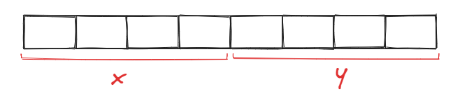
\includegraphics[width=7cm]{images/inisialisasi populasi_1.png}
    \caption{Ilustrasi Individu}
    \label{fig:individu}
\end{figure}

Setiap biner yang tercatat pada masing-masing gen akan merepresentasikan parameter untuk fitur-fitur yang diterapkan.\cite{Hussein2020} Untuk menerapkan fungsi pengenalan objek, umumnya setiap biner memiliki parameter untuk mengelompokkan pola dalam pixel sebuah gambar objek. Dalam penerapan pengenalan wajah, dipertimbangkan ukuran gambar dalam file database 64x64 pixel. Dengan demikian, dapat diberikan setiap solusi yang dihasilkan oleh chromosome akan mewakili posisi (x, y) dari kelompok-kelompok pixel posisi gambar. Dari gambaran tersebut, dapat diberikan panjang kromosom 8 bit, dengan 4 bit untuk koordinat x, dan 4 bit untuk koordinat y.

Populasi didefinisikan sebagai kumpulan subset dari semua kemungkinan solusi (encoded) untuk masalah yang dipecahkan. \cite{Champlin2018}. Populasi dapat dianalogikan sebagai kumpulan banyak kandidat individu yang memiliki solusinya masing-masing untuk memecahkan masalah. \cite{Hijriana2015}

\begin{figure}[htp]
    \centering
    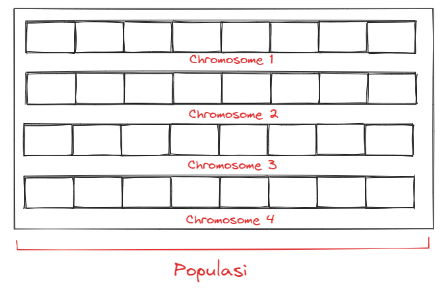
\includegraphics[width=7cm]{images/inisialisasi populasi_2.png}
    \caption{Ilustrasi Populasi}
    \label{fig:populasi}
\end{figure}

Pada pemecahan masalah saat ini, populasi diperoleh dengan menganggap telah memiliki populasi diperoleh acak yang dianalogikan sebagai dataset gambar untuk melatih pengenalan wajah. Pendekatan teori yang digunakan yaitu inisialisasi acak untuk inisiasi awal populasi. Dengan menetapkan setiap populasi akan diisi dengan 4 kelas chromosome pada masing-masing generasi, maka telah diperoleh data yang dapat digunakan untuk melakukan pengujian dengan Genetic Algorithm.

\subsection{Fungsi Fitness}

Tahap ini akan mengevaluasi setiap individu dari populasi yang tersedia. Setiap individu akan dievaluasi menggunakan suatu fungsi yang telah disesuaikan dengan metode dan kriteria pemecahan masalah. \cite{Marleny2019}. Tahap evaluasi fitnes ini dapat disesuaikan dengan kebutuhan dan akan terus berjalan sampai kriteria kesuksesan yang telah ditetapkan berhenti.

\begin{figure}[htp]
    \centering
    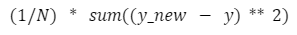
\includegraphics[width=7cm]{images/formula_fitness.png}
    \caption{Rumus Fitness}
    \label{fig:fitness}
\end{figure}

Mean Squared Error (MSE) dapat digunakan sebagai model matrix yang umum digunakan untuk pengujian mengevaluasi fitnes model pengenalan wajah. \cite{Hussein2020}. Pada Fig. \ref{fig:fitness} diambil fungsi pengujian untuk MSE dengan mengambil kuadrat selisih antara nilai prediksi dan nilai sebenarnya, lalu merata-ratakan semua titik data. Parameter `y` diperoleh dari chromosome yang telah diberikan di awal. Kemudian akan dibandingkan dengan metrik dari `y-new` yang merupakan hasil dari nilai yang disimpan untuk menyimpan nilai target yang diprediksi untuk input fitur baru. Perolehan MSE yang semakin rendah akan menghasilkan pengujian yang dapat dinilai baik untuk kecocokan model.

\subsection{Operasi Penyilangan Genetika}

Parent selection digunakan pada genetic algorithm untuk menentukan individu dari populasi saat ini yang akan disilangkan sebagai parent untuk melahirkan generasi baru atau sebagai offspring. Tujuan dari tahap ini pada genetic algorithm yaitu untuk menghasilkan solusi yang lebih baik lagi dengan terus melahirkan individu dengan nilai fitnes yang lebih tinggi. Oleh karena itu, parent selection merupakan tahap yang krusial pada metode optimasi genetic algorithm.

\begin{center} p=fitness-values / sum(fitness-values) \end{center}

\begin{figure}[htp]
    \centering
    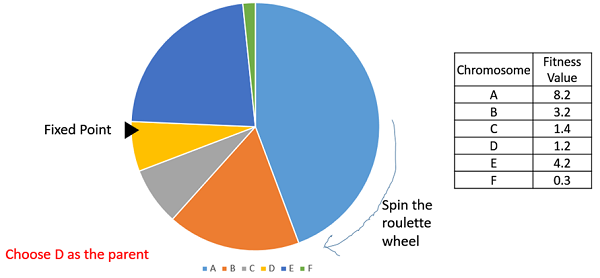
\includegraphics[width=8cm]{images/roulette_wheel_selection.jpg}
    \caption{Ilustrasi Roulette Wheel Selection}
    \label{fig:parent}
\end{figure}

Pada percobaan kali ini digunakan metode roulette wheel yang menggunakan nilai acak sebagai acuannya untuk menghasilkan parent dari individu hasil Evaluate Fitness. Probabilitas pemilihan untuk kandidat parent dipilih dengan menggunakan persamaan Fig. \ref{fig:parent} yang akan mengkalkulasikan nilai fitness. Hal tersebut diperkirakan akan menghasilkan peluang yang proporsional untuk individu dengan nilai fitness yang lebih tinggi untuk dipilih sebagai parent.

Crossover merupakan proses yang menggabungkan parent atau individu yang telah dipilih untuk digabungkan dengan tujuan untuk menghasilkan individu-individu baru. Dengan menjalankan crossover, individu baru akan menghasilkan solusi-solusi baru untuk menyelesaikan masalahnya. 

\begin{figure}[htp]
    \centering
    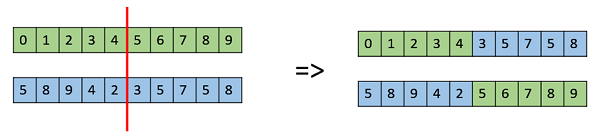
\includegraphics[width=8cm]{images/one_point_crossover.jpg}
    \caption{Ilustrasi One Point Crossover}
    \label{fig:crossover}
\end{figure}

Metode crossover yang akan digunakan pada penelitian ini adalah single-point crossover. Metode tersebut akan menyilangkan kedua kandidat individu dengan menentukan titik potong secara acak. \cite{Ertel2011} Setelah titik pemotongan crossover ditentukan, gen-gen sebelum titik pemotongan dari parent A dan gen-gen setelah titik pemotongan dari parent B digabungkan untuk membentuk offspring pertama. Gen-gen sebelum titik pemotongan dari parent B dan gen-gen setelah titik pemotongan dari parent A digabungkan untuk membentuk offspring kedua.

\subsection{Operasi Mutasi Genetika}

Mutation merupakan proses mengubah nilai dari satu atau beberapa gen dalam suatu kromosom. Pemberlakukan mutation ini adalah untuk menggantikan gen yang hilang dari populasi akibat proses seleksi yang memungkinkan munculnya kembali gen yang tidak muncul pada inisialisasi populasi.

Bit-flip mutation merupakan metode yang digunakan pada percobaan kali ini. Dalam bit-flip mutation, setiap gen dalam individu memiliki peluang untuk mengalami mutasi. Jika nilai acak yang dihasilkan kurang dari mutation rate yang telah ditentukan, gen tersebut akan mengalami perubahan nilainya, yaitu flip dari 0 menjadi 1 atau sebaliknya.

Proses-proses yang telah dilakukan sebelumnya kemudian akan diulang kembali hingga sampai ke target generasi yang diinginkan. Setiap mutasi generasi akan menghasilkan tingkat kesuksesan yang berbeda berhubungan dengan mutasi generasi yang memiliki nilai evaluate fitness yang baik. Siklus tidak hanya berpaku pada batas generasi yang telah ditentukan, melainkan siklus dapat berlangsung hingga kondisi solusi yang memadai terbentuk.

Pada metode yang diterapkan kali ini, siklus akan terus berulang hingga generasi ke-10. Hal tersebut akan menguji tingkat keberhasilan genetic algorithm dalam mengoptimasi nilai yang diharapkan. Proses ini melibatkan penggunaan teknik genetic algorithm yang melibatkan konsep seleksi, persilangan, dan mutasi. 

\subsection{Optimasi Metode}

Pada penelitian sebelumnya yang dilakukan oleh Pratibha Sukhija, dkk. metode pendekatan optimasi algortima yang digunakan dibagi menjadi 3 cara, yaitu Genetic Algorithm, Principal Component Analisys (PCA), dan Linear Discriminant Analysis (LDA). \cite{Sukhija2016}. Perbandingan tersebut menampilkan data yang bervariasi pada setiap cara yang diterapkan.

PCA yang merupakan metode statistik yang digunakan untuk menganalisis hubungan antara variabel-variabel dalam sebuah dataset. Tujuan dari PCA adalah untuk mengidentifikasi pola tersembunyi, mengurangi dimensi data, dan memvisualisasikan data yang kompleks dalam bentuk yang lebih sederhana. Dengan demikian,  PCA membantu dalam mengurangi dimensi data dengan mempertahankan sebagian besar informasi yang ada dalam dataset.

LDA adalah sebuah metode statistik yang digunakan dalam analisis data untuk membedakan atau mengklasifikasikan pengamatan ke dalam dua atau lebih kelompok berdasarkan variabel prediktor. Tujuan dari LDA adalah untuk mencari kombinasi linear dari variabel prediktor yang memiliki kemampuan terbaik dalam membedakan atau mengklasifikasikan kelompok-kelompok tersebut. Dalam LDA, kita mencari linear discriminant functions (fungsi pemisah linear) yang dapat memaksimalkan jarak antara pusat kelompok dan meminimalkan variasi dalam kelompok. 




\section{Pembahasan}

\subsection{Percobaan Genetika Algoritma}

Metode percobaan genetika algoritma direkayasa menggunakan bahasa pemrograman python dengan menggunakan dataset yang diinisiasi di awal. Inisiasi populasi ditargetkan hingga 20 individu dengan batasan hingga 100 generasi. Tingkat mutasi dibatasi hingga 0.1 untuk menjaga variasi genetik dalam populasi dan mempertahankan informasi yang bernilai.

\begin{figure}[htp]
    \centering
    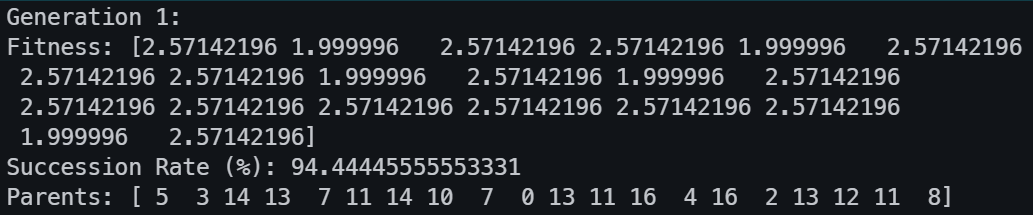
\includegraphics[width=8cm]{images/Generation 1.png}
    \caption{Generasi 1}
    \label{fig:Generation1}
\end{figure}

Percobaan pada generasi pertama pada (figure generasi 1) menghasilkan tingkat akurasi keberhasilan hingga 94.4% setelah melalui tahapan genetika algoritma. Generasi akan terus berlanjut hingga generasi ke-100 untuk menghasilkan tingkat akurasi yang lebih akurat. Setelah melalui proses, dihasilkan generasi ke-100 sebagai berikut.

\begin{figure}[htp]
    \centering
    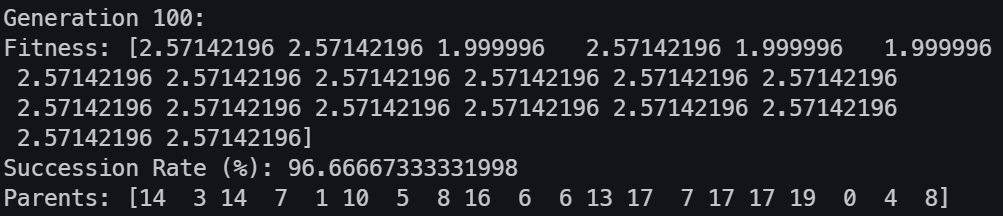
\includegraphics[width=8cm]{images/Generation 100.png}
    \caption{Generasi 100}
    \label{fig:Generation100}
\end{figure}

Generasi ke-100 telah mengalami peningkatan akurasi yang lebih baik hingga angka 96.6% meningkat hingga 2.2% dari generasi pertama. Meski demikian, dikarenakan populasi yang terbatas, beberapa individu parent yang ditetapkan pada generasi pertama masih mengikuti hingga generasi ke-100. Hal lain yang didapati yaitu, pada beberapa generasi terjadi penurunan yang tidak terlalu signifikan hingga menyentuh persentase akurasi paling rendah 90%. 

\begin{figure}[htp]
    \centering
    
\includegraphics[width=7cm]{images/MSE.png}
    \caption{Fitness and Chromosome}
    \label{fig:MSE}
\end{figure}

Dari analisis keseluruhan genetika algoritma, dihasilkan angka terbaik untuk fungsi fitness hingga 0.518 dan chromosome terbaik [1 0 0 0]. Hasil tersebut dapat membantu untuk mengembangkan kembali algoritma yang diterapkan untuk percobaan berikutnya. Persentase akurasi dari algoritma genetika pada percobaan ini konsisten menghasilkan tingkat akurasi lebih dari 90\%. Dengan demikian genetika algoritma dapat digunakan untuk optimasi pengenalan biometrik dan objek untuk meningkatkan keamanan sistem komputer.

\subsection{Percobaan Metode Pengenalan Objek}

Hasil percobaan dari metode algoritma genetika yang diterapkan dapat diperkuat dengan perbandingan hasil dengan penelitian terdahulu dan metode-metode pembanding. Dari metode yang diterapkan, dihasilkan metode pembanding genetika algoritma dari metode statistik PCA dan LDA. Dari jurnal yang dipublikasikan oleh Pratibha Sukhija, Sunny Behal dan Pritpal Singh mereka mendapati beberapa keunggulan dengan menerapkan metode Genetika Algoritma. \cite{Sukhija2016}.

\begin{figure}[htp]
    \centering
    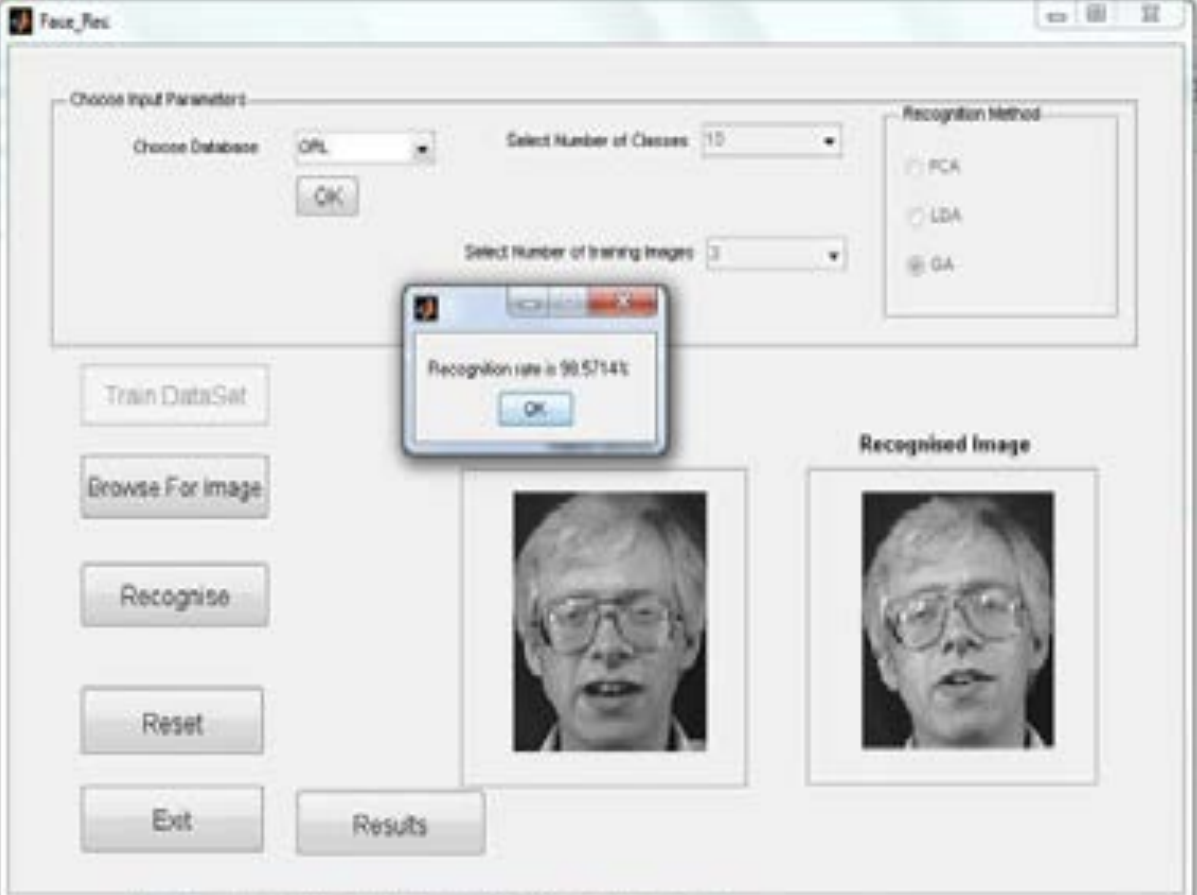
\includegraphics[width=5cm]{images/percobaan_fig1.png}
    \caption{Percobaan 1}
    \label{fig:percobaan1}
\end{figure}

\begin{figure}[htp]
    \centering
    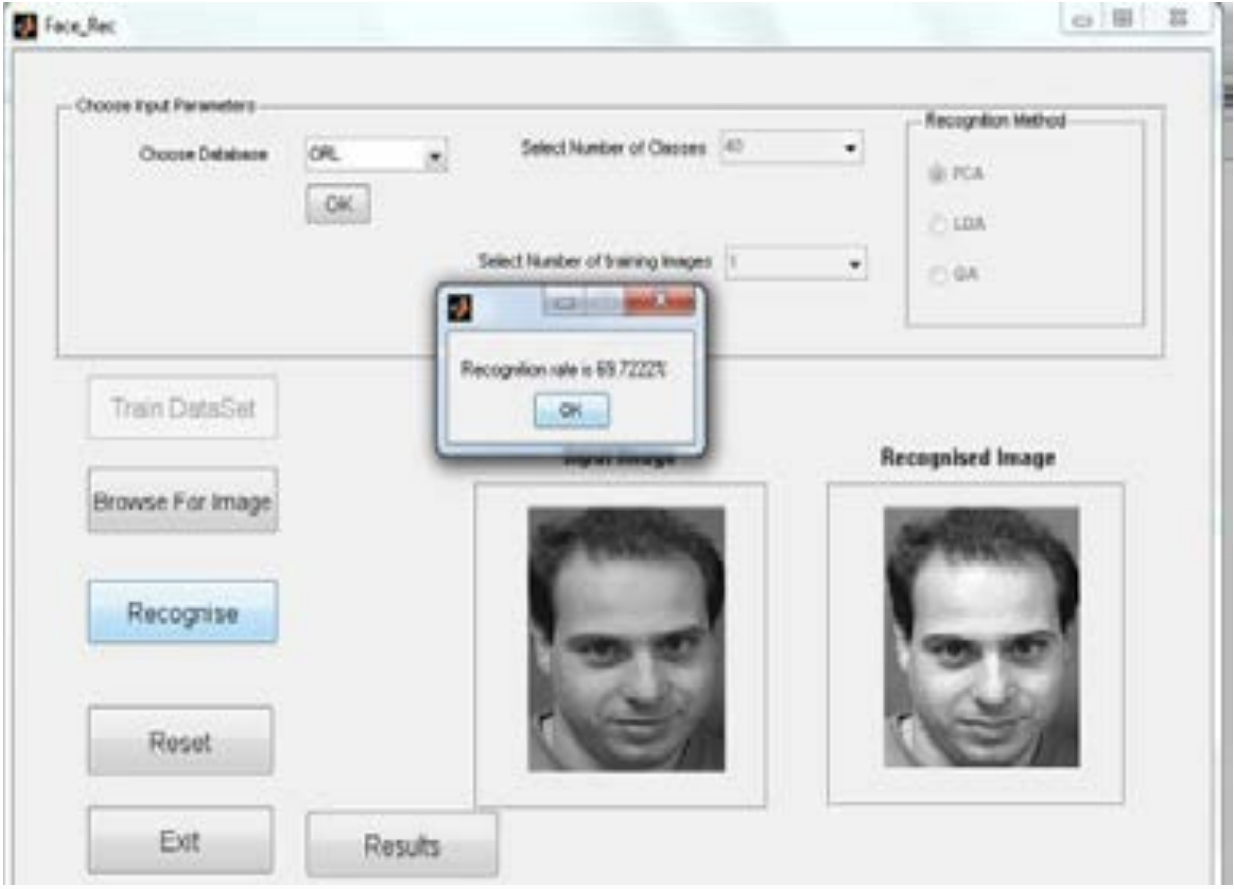
\includegraphics[width=5cm]{images/percobaan_fig2.png}
    \caption{Percobaan 2}
    \label{fig:percobaan2}
\end{figure}

\begin{figure}[htp]
    \centering
    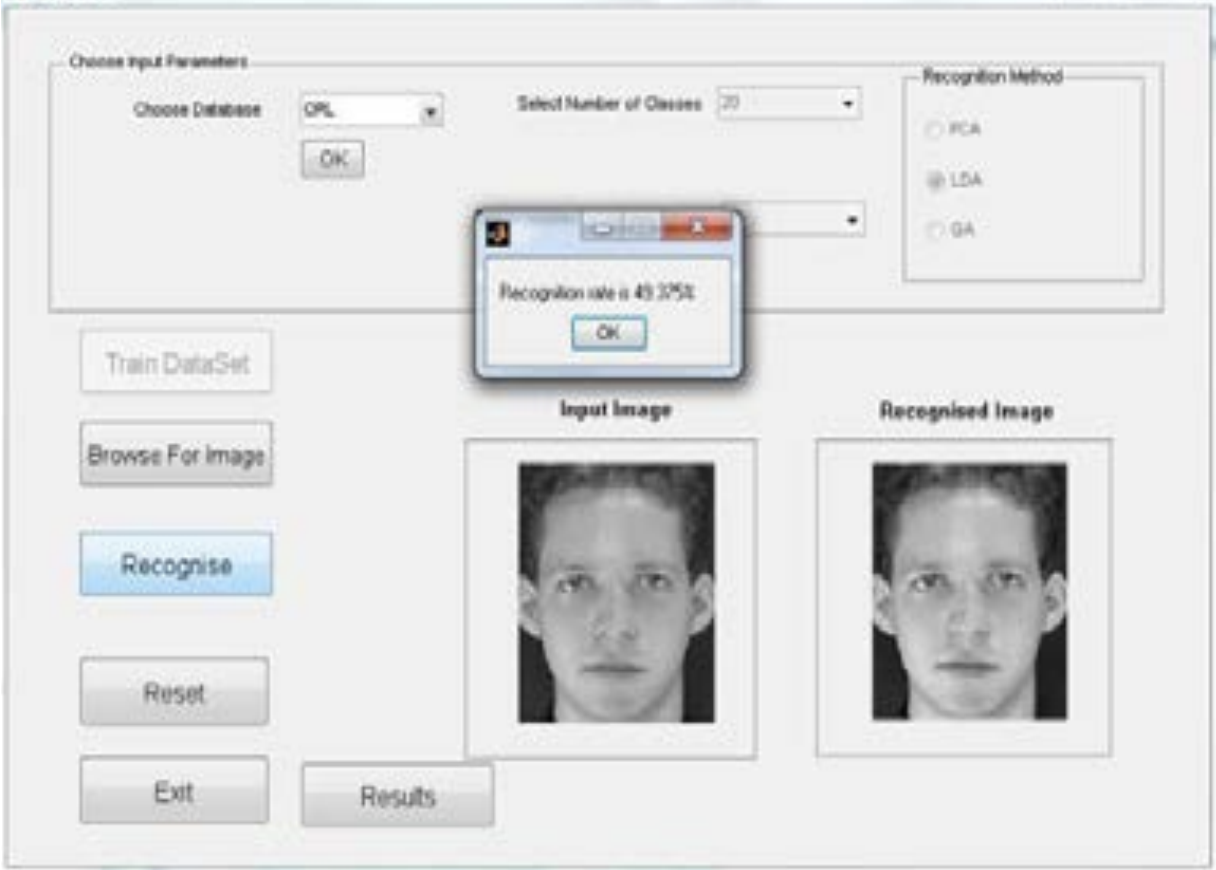
\includegraphics[width=5cm]{images/percobaan_fig3.png}
    \caption{Percobaan 3}
    \label{fig:percobaan3}
\end{figure}

Figures percobaan menunjukkan hasil dari perbandingan tiga metode berbeda yang telah diterapkan. Perbandingan tersebut menunjukkan percobaan aplikasi pengenalan wajah dengan tingkat akurasinya masing-masing. Figure \ref{fig:percobaan1} menunjukkan tingkat akurasi ketepatan dengan angka persentase 90.5\% dari gambar yang dimasukkan. Figure \ref{fig:percobaan2} menunjukkan tingkat akurasi ketepatan dengan angka persentase 69\% dari gambar yang dimasukkan. Dan, figure \ref{fig:percobaan3} menunjukkan tingkat akurasi ketepatan dengan angka persentase 49\% dari gambar yang dimasukkan. Percobaan sederhana tersebut menunjukkan genetika algoritma yang memiliki tingkat akurasi tertinggi dari metode-metode lainnya.

Setelahnya percobaan dilakukan kembali dengan menambahkan database yang menyimpan kumpulan gambar wajah untuk dilakukan percobaan pada ketiga metode yang diuji. Database diambil dari Olivetti Research Laboratory (ORL), University of Manchester Institute of Science and Technology (UMIST), dan Indian Face Database (Indbase). Setiap database kemudian diuji dengan kelas populasi dan percobaan dengan rubrik yang berbeda pada setiap iterasinya.

    \begin{table}[htbp!]
    \small % Reduce font size
    \centering
    \setlength{\tabcolsep}{6pt} % Reduce column width
    \renewcommand{\arraystretch}{2.2} % Adjust vertical spacing
    \begin{tabular}{|c|c|c|c|c|}
    \hline
    Method & Database & Classes & Test Cases & Rate \\ \hline
    \multirow{4}{*}{GA} & \multirow{4}{*}{ORL} & 10 & 3 & 98.58 \\
    & & 20 & 4 & 97.5 \\
    & & 30 & 8 & 95.00 \\
    & & 40 & 7 & 92.50 \\ \hline
    \multirow{3}{*}{GA} & \multirow{3}{*}{UMIST} & 10 & 6 & 97.50 \\
    & & 10 & 7 & 100.00 \\
    & & 20 & 7 & 91.66 \\ \hline
    \multirow{3}{*}{GA} & \multirow{3}{*}{Indbase} & 10 & 4 & 98.33 \\
    & & 10 & 5 & 98.00 \\
    & & 20 & 6 & 96.00 \\ \hline
    \end{tabular}
    
    \caption{Genetic Algorithm Method}
    \end{table}
    

    \begin{table}[htbp!]
    \small % Reduce font size
    \centering
    \setlength{\tabcolsep}{6pt} % Reduce column width
    \renewcommand{\arraystretch}{2.2} % Adjust vertical spacing
    \begin{tabular}{|c|c|c|c|c|}
    \hline
    Method & Database & Classes & Test Cases & Rate \\ \hline
    \multirow{4}{*}{PCA} & \multirow{4}{*}{ORL} & 10 & 3 & 97.14 \\
    & & 20 & 4 & 91.44 \\
    & & 30 & 3 & 87.60 \\
    & & 40 & 2 & 81.87 \\ \hline
    \multirow{3}{*}{PCA} & \multirow{3}{*}{UMIST} & 10 & 2 & 73.75 \\
    & & 10 & 2 & 70.62 \\
    & & 20 & 4 & 84.16 \\ \hline
    \multirow{3}{*}{PCA} & \multirow{3}{*}{Indbase} & 10 & 3 & 58.71 \\
    & & 10 & 4 & 60.00 \\
    & & 20 & 5 & 70.00 \\ \hline
    \end{tabular}
    
    
    \caption{Genetic Algorithm Method}
    \end{table}

    \begin{table}[htbp!]
    \small % Reduce font size
    \centering
    \setlength{\tabcolsep}{6pt} % Reduce column width
    \renewcommand{\arraystretch}{2.2} % Adjust vertical spacing
    \begin{tabular}{|c|c|c|c|c|}
    \hline
    Method & Database & Classes & Test Cases & Rate \\ \hline
    \multirow{4}{*}{LDA} & \multirow{4}{*}{ORL} & 10 & 2 & 76.25 \\
    & & 20 & 4 & 55.00 \\
    & & 30 & 4 & 42.70 \\
    & & 40 & 2 & 36.25 \\ \hline
    \multirow{3}{*}{LDA} & \multirow{3}{*}{UMIST} & 10 & 2 & 28.75 \\
    & & 10 & 2 & 63.12 \\
    & & 20 & 4 & 60.83 \\ \hline
    \multirow{3}{*}{LDA} & \multirow{3}{*}{Indbase} & 10 & 2 & 52.5 \\
    & & 10 & 3 & 70.00 \\
    & & 20 & 4 & 33.33 \\ \hline
    \end{tabular}
    
    \caption{Genetic Algorithm Method}
    \end{table}

Rubrik diatas mengindikasikan tingkat akurasi pada masing-masing metode yang diterapkan. Dengan demikian, dihasilkan tingkat ketepatan akurasi yang beragam untuk masing-masing metode yang diterapkan. Berdasarkan rubrik-rubrik yang diterapkan sebelumnya, maka dihasilkan visualisasi data sebagai berikut.\\ \\ \\

\begin{figure}[htp]
    \centering
    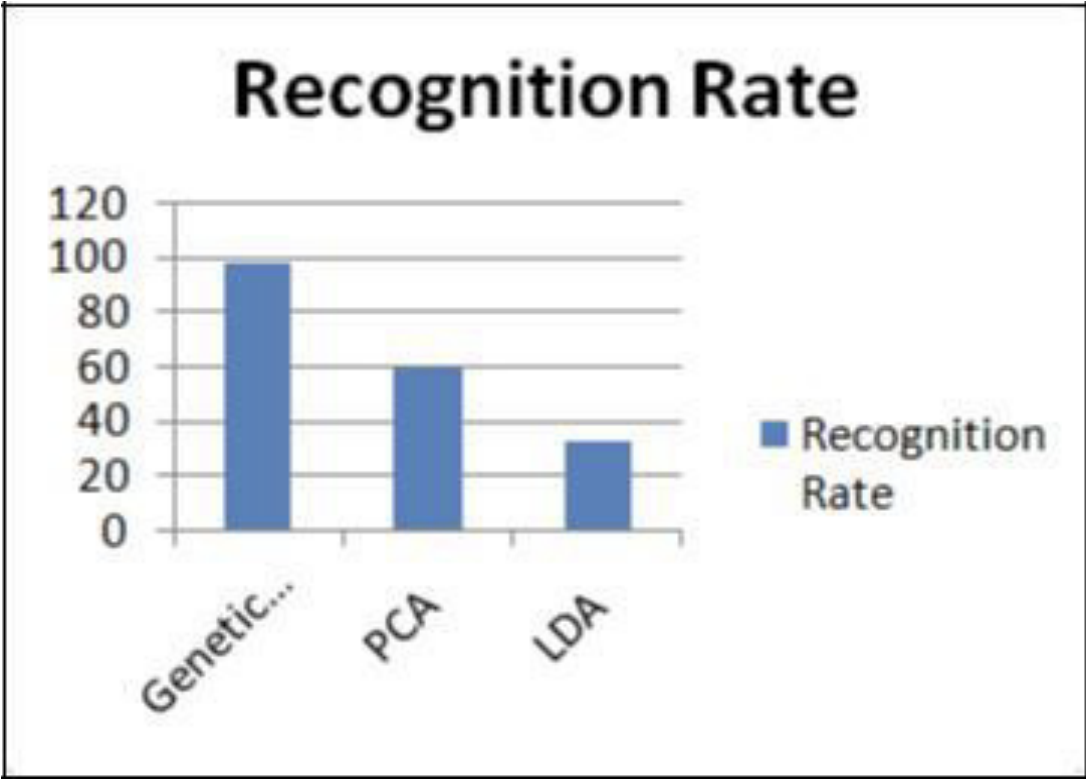
\includegraphics[width=7cm]{images/CHA1.png}
    \caption{Chart 1}
    \label{fig:ORL}
\end{figure}

\begin{figure}[htp]
    \centering
    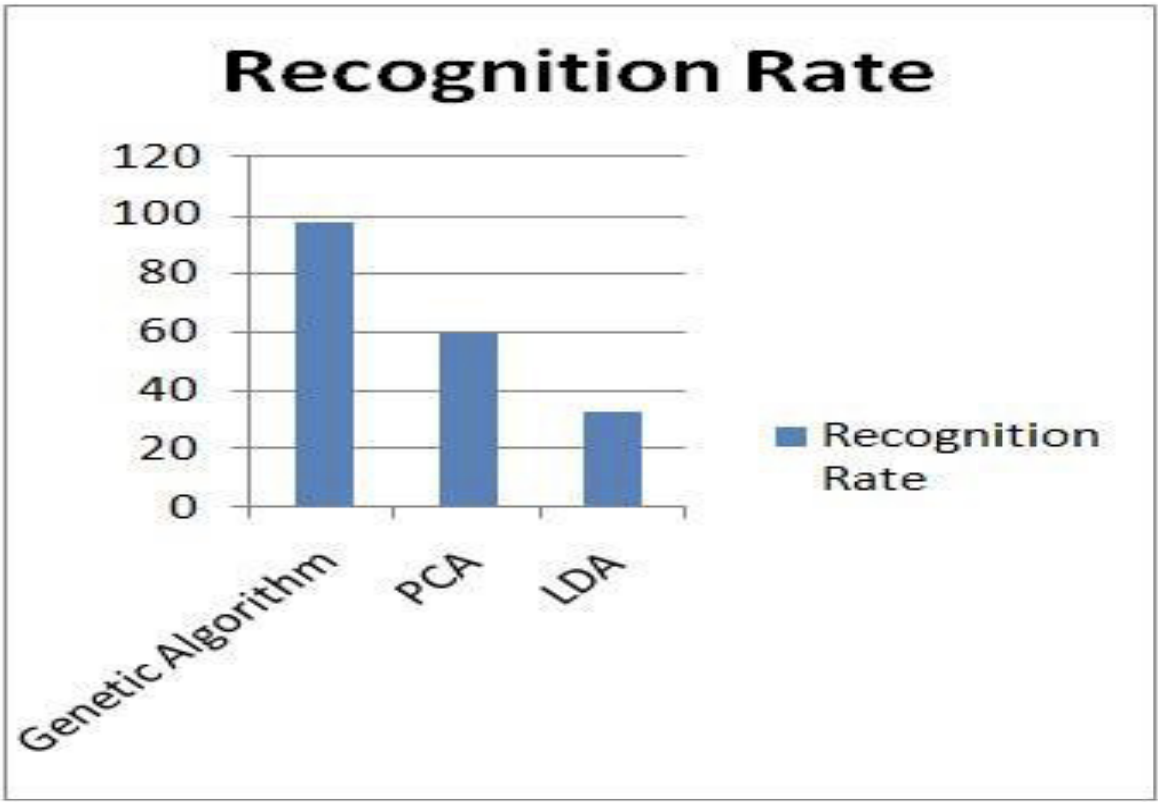
\includegraphics[width=7cm]{images/CHA2.png}
    \caption{Chart 2}
    \label{fig:UMIST}
\end{figure}

\begin{figure}[htp]
    \centering
    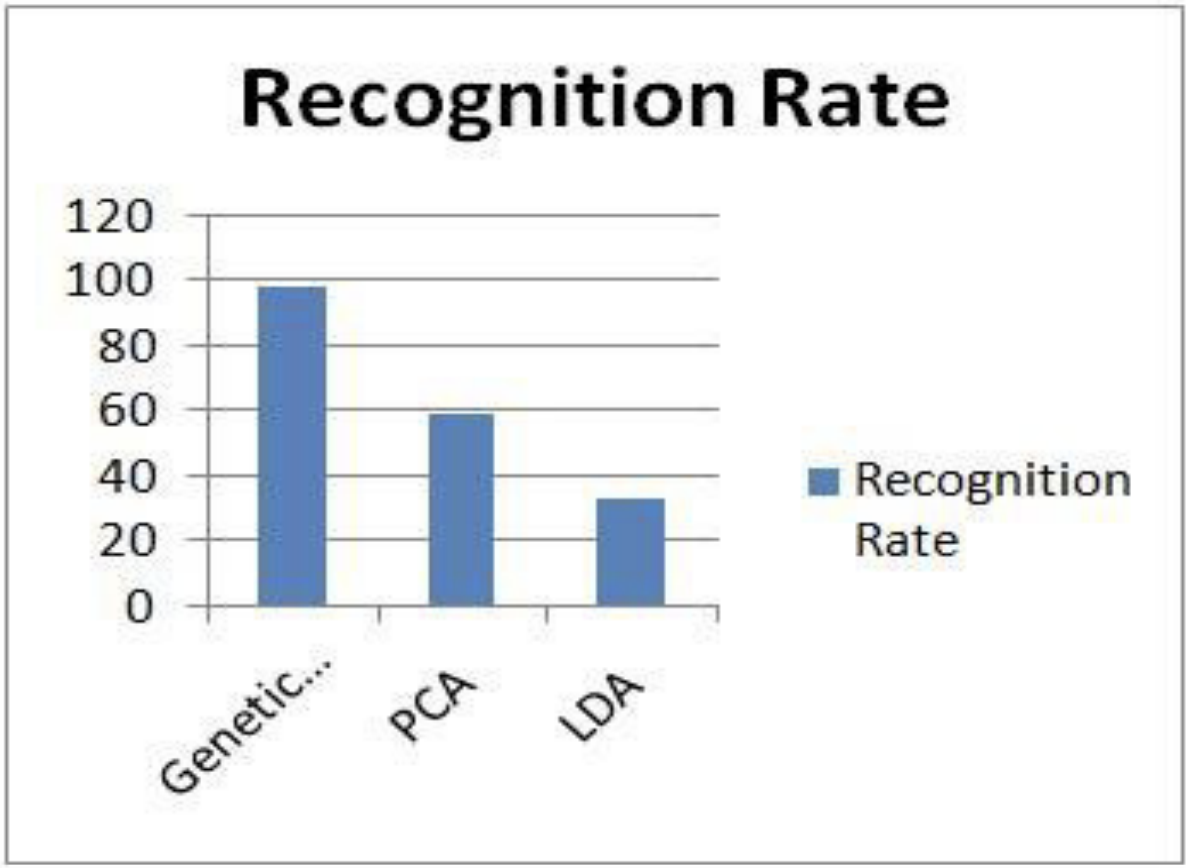
\includegraphics[width=7cm]{images/CHA3.png}
    \caption{Chart 3}
    \label{fig:INDBASE}
\end{figure}

Figure tersebut menampilkan tingkat pengenalan wajah pada masing database yang digunakan. Tingat akurasi terendah dihasilkan oleh metode LDA dengan akurasi pengenalan tidak lebih dari persentase 40\%. Sedangkan untuk tingkat akurasi tertinggi diperoleh genetika algoritma dengan akurasi pengenalan lebih dari 90\%.

\section{Analysis}

Setelah selesai menguji dan membandingkan hasil dengan metode penelitian terdahulu dihasilkan kesimpulan untuk masing-masing metode yang diterapkan. Analisis yang dihasilkan metode-metode yang diuji memungkinkan penerapannya pada sistem keamanan komputer. Pendekatan yang paling memungkinkan dapat diterapkan dengan menyesuaikan dengan hasil pengujian. 

Pengenalan biometrik sebagai sistem keamanan komputer dapat diterapkan menggunakan optimasi genetika algoritma. Hal tersebut dibuktikan dari hasil pengujian mandiri penulis dan pengujian penelitian terdahulu. Kedua hasil pengujian tersebut menghasilkan tingkat akurasi yang konsisten. Genetika algoritma menghasilkan tingkat akurasi lebih dari 90\% untuk mengenali biometrik. Dengan demikian, penerapannya untuk keamanan komputer sangat memungkinkan untuk dilakukan.

\section{Discussion}
Komputer dan kecerdasan buatan memainkan peran penting dalam kehidupan manusia saat ini, namun juga menghadirkan tantangan keamanan di dunia digital. Penerapan sistem keamanan dengan kecerdasan buatan berbasis algoritma genetik dan pengenalan citra menjadi pendekatan menjanjikan untuk meningkatkan keamanan komputer. Face recognition dapat diterapkan dalam berbagai bidang keamanan digital. Tantangan dalam face recognition meliputi variasi struktural wajah, posisi, ekspresi, penyensoran, orientasi gambar, kondisi pemotretan, dan perubahan akibat usia. Meski demikian, metode biometrik ini menawarkan keunggulan dalam mengenali individu berdasarkan karakteristik fisiologis yang sulit dipalsukan. 

Penelitian ini menunjukkan tingkat akurasi pengenalan wajah dengan pengujian dan kajian literatur untuk metode Genetika Algoritma, PCA, dan LDA. Setelah dilakukan metode-metode penelitian, genetika algoritma memiliki kemungkinan tertinggi untuk diterapkan pada sistem keamanan biometrik. Pengujian yang dilakukan penulis dan pengujian genetika algoritma oleh Pritpal Singh dan Sunny Behal memiliki tingkat akurasi yang hampir seimbang.

Kebutuhan data variasi wajah sangat mempengaruhi tingkat akurasi pengujian metode. Oleh karena itu, pada pengujian selanjutnya sangat disarankan untuk mempertimbangkan ketepatan kebutuhan data yang dimiliki. Selain itu, rubrik-rubrik yang dapat menjadi parameter pengujian memiliki kompleksitas berbeda-beda dan memiliki kesesuaian yang beragam untuk masing-masing metode. Parameter tersebut menjadi hal yang krusial untuk meningkatkan tingkat akurasi pengujian. \cite{Katoch2021} Perbaikan-perbaikan ini diharapkan menghasilkan pengujian dan tingkat akurasi yang lebih akurat untuk penelitian selanjutnya.


\bibliographystyle{IEEEtran}
\bibliography{biblio}
\end{document}
